%\documentclass[sigconf, authordraft]{acmart}
\documentclass[sigconf]{acmart}
\usepackage{algpseudocode,algorithm}
\usepackage{hyperref}
\usepackage{listings}
\usepackage{xcolor}
\usepackage{xstring}
\usepackage{wasysym}
\usepackage{MnSymbol}
\usepackage{booktabs} % For formal tables
\graphicspath{ {./images/} }

\definecolor{NavyBlue}{HTML}{000080}
\definecolor{Magenta}{HTML}{FF00FF}
\definecolor{Orange}{HTML}{FFA500}
\definecolor{CornflowerBlue}{HTML}{6495ED}
\definecolor{YellowGreen}{HTML}{9ACD32}
\definecolor{Gray}{HTML}{BEBEBE}
\definecolor{Yellow}{HTML}{FFFF00}
\definecolor{GreenYellow}{HTML}{ADFF2F}
\definecolor{ForestGreen}{HTML}{228B22}
\definecolor{Lavender}{HTML}{FFC0CB}
\definecolor{SkyBlue}{HTML}{87CEEB}
\definecolor{NavyBlue}{HTML}{000080}
\definecolor{Goldenrod}{HTML}{DDF700}
\definecolor{VioletRed}{HTML}{D02090}
\definecolor{CornflowerBlue}{HTML}{6495ED}
\definecolor{LimeGreen}{HTML}{32CD32}


% Copyright
%\setcopyright{none}
%\setcopyright{acmcopyright}
%\setcopyright{acmlicensed}
\setcopyright{rightsretained}
%\setcopyright{usgov}
%\setcopyright{usgovmixed}
%\setcopyright{cagov}
%\setcopyright{cagovmixed}


% DOI
\acmDOI{10.1145/nnnnnnn.nnnnnnn}

% ISBN
\acmISBN{978-x-xxxx-xxxx-x/YY/MM}

% Conference
\acmConference[GECCO '20]{the Genetic and Evolutionary Computation Conference 2020}{July 8--12, 2020}{Cancun, Mexico}
\acmYear{2020}
\copyrightyear{2020}

%\acmArticle{4}
\acmPrice{15.00}

% These commands are optional
%\acmBooktitle{Transactions of the ACM Woodstock conference}
%\editor{Jennifer B. Sartor}
%\editor{Theo D'Hondt}
%\editor{Wolfgang De Meuter}


\begin{document}
\title{Event-driven multi-population optimization: mixing Swarm and Evolutionary strategies}
%\titlenote{Produces the permission block, and copyright information}
%\subtitle{Subtitle}
%\subtitlenote{The full version of the author's guide is available as
%  \texttt{acmart.pdf} document}

%%% The submitted version for review should be ANONYMOUS
\author{ANONYMOUS}
\authornote{Dr.~ANONYMOUS insisted his name be first.}
\orcid{1234-5678-9012}
\affiliation{%
  \institution{Institute for Clarity in Documentation}
  \streetaddress{P.O. Box 1212}
  \city{Dublin} 
  \state{Ohio} 
  \postcode{43017-6221}
}
\email{ANONYMOUS@ANONYMOUS.com}


\author{ANONYMOUS ANONYMOUS}
\affiliation{%
  \institution{ANONYMOUS Research Laboratories}
  \streetaddress{8600 Datapoint Drive}
  \city{ANONYMOUS ANONYMOUS}
  \state{ANONYMOUS} 
  \postcode{78229}}
\email{ANONYMOUS@ANONYMOUS.com}




% The default list of authors is too long for headers.
\renewcommand{\shortauthors}{ANONYMOUS et al.}

\begin{abstract}
  Recently, in the field of nature-inspired optimization, 
  researchers have proposed multi-population asynchronous 
  algorithms that distribute the evolutionary process among 
  heterogeneous search paradigms.These algorithms execute 
  the search strategy by reading streams of populations 
  from message queues, and replacing them with evolved versions of them.
  Moreover, current studies suggest that when we have a high number of populations
  interacting in parallel, the effect of the individual parameters
  of each population is compensated by those selected in other
  populations, 
  improving the overall performance of the algorithm. In this work,
  we propose a simple reactive migration method for the 
  asynchronous execution of multi-population, multi-strategy 
  algorithms that improves over homogeneous configurations.
  We evaluate this method by comparing between % with? 
  homogeneous and an ensemble of 
  multi-populations, using Genetic Algorithms (GAs) and Particle 
  Swarm Optimization (PSO) in the noiseless BBOB testbed for 
  the optimization of continuous functions. Results show,
  that this method offers better performance, even when compared
  with other asynchronous population based algorithms. 
\end{abstract}

%
% The code below should be generated by the tool at
% http://dl.acm.org/ccs.cfm
% Please copy and paste the code instead of the example below. 
%
% REmember to change this - JJ
% Done - Mario
\begin{CCSXML}
  <ccs2012>
  <concept>
  <concept_id>10003752.10003809.10003716.10011138.10011803</concept_id>
  <concept_desc>Theory of computation~Bio-inspired optimization</concept_desc>
  <concept_significance>500</concept_significance>
  </concept>
  <concept>
  <concept_id>10010520.10010521.10010537.10003100</concept_id>
  <concept_desc>Computer systems organization~Cloud computing</concept_desc>
  <concept_significance>500</concept_significance>
  </concept>
  <concept>
  <concept_id>10010147.10010919.10010172</concept_id>
  <concept_desc>Computing methodologies~Distributed algorithms</concept_desc>
  <concept_significance>500</concept_significance>
  </concept>
  </ccs2012>
\end{CCSXML}
  
  \ccsdesc[500]{Theory of computation~Bio-inspired optimization}
  \ccsdesc[500]{Computer systems organization~Cloud computing}
  \ccsdesc[500]{Computing methodologies~Distributed algorithms}

\keywords{heterogeneous multi-population algorithms, genetic algorithms, particle swarm optimization, cloud-native systems}


\maketitle

\section{Introduction}

Nature-inspired optimization algorithms have been used successfully in the last
decades to tackle complex problems \cite{yang2014nature}. These
algorithms include evolutionary algorithms (EAs)
\cite{back1996evolutionary} and swarm intelligence (SI)
\cite{kennedy2006swarm}. % Maybe mention a few more, like bee o others
                         % like that? - JJ
Genetic Algorithms (GAs) 
\cite{holland1992adaptation,eiben2003genetic}, and
Differential Evolution (DE) \cite{karabouga2004simple} are two popular
EAs, while examples of SI algorithms 
\cite{kennedy2006swarm} are particle swarm optimization (PSO)
\cite{clerc2010particle}, and ant colony algorithms (ACO) \cite{dorigo1999ant}.
A common characteristic of these kind of methods is the
use of an initial set of random candidate solutions that are manipulated by the
algorithm to generate a new set of candidates, and because of this, we commonly
referred to them as population-based algorithms. % There are other
                                % population based algorithms that are
                                % not natural, such as PBIL. Maybe you
                                % could mention them - JJ

Since instead of piecewise constructing a population or changing it
incrementally, all members of the population have to be evaluated to
obtain a fitnen of each population.  In this paper, we are interested in the
latter, that is, having multiple populations running with distinct parameters
and optimization algorithms. We can find in the literature, several
heterogeneous e it is difficult to overcome that $n$ factor, where $n$
is the population size, in the complexity of every iteration of the
algorithm. That is why researchers have been proposing some form of
parallelization since early on \cite{muhlenbein1988evolution} to
increase their scalability. % Not scalability, but wallclock timing - JJ
One of the first methods of parallelization was the island
model, which lead to an increased performance
\cite{gorges1990explicit,grosso1985computer}. The concept was to divide the
population into smaller populations that communicated with each other. Other
population-based algorithms have adopted the technique, and since then,
researchers have found additional advantages besides the execution speed, 
these include avoiding a premature convergence and maintaining the diversity of the
global population \cite{li2015multi}, we are going to call these methods 
multi-population algorithms \cite{Ma2019}. The relative 
isolation in which populations carry out the algorithm, together with the
synchronous or asynchronous communication, helps to increase the overall
diversity since each population will search in a particular area, at least
between communications. Multi-population algorithms use a form of
communication to recombine or migrate candidate solutions between populations
to avoid premature convergence, since smaller populations are known to perform
better for a given problem than bigger populations
\cite{li2016multi,wu2016differential}.  Even in some cases, a multi-population based
algorithm scales better due to these interactions, and the parallelism of the
operation \cite{ALBA20027}. 

Having many populations offers researchers many configuration options and
additional challenges when designing efficient multi-population algorithms.
Options include the number and size of populations, the interaction between
them, the search area of each population, and the search strategy and
parametrization of each population.  In this paper, we are interested in the
latter, that is, having multiple populations running with distinct parameters
and optimization algorithms. We can find in the literature, several
heterogeneous multi-population algorithms integrating variations of optimization
algorithms, and these often perform better than single-population or homogeneous
multi-population optimization algorithms\cite{wu2016differential,nseef2016adaptive}.
Heterogeneous algorithms add to
the problem of finding the correct parameter settings for each population;
because some parameters affect the accuracy of the solution and the convergence
speed of the individual algorithms as they tip the balance between exploration
and exploitation of the search space. On the other hand, current studies show
that by having a high number of populations communicating in parallel, the
effect of the individual parameters of each population is compensated by those
selected in other populations \cite{li2016multi,tanabe2013evaluation}. Some
level of heterogeneity can be implemented by just changing the configuration
parameters of each population, but in this case, we are interested in
heterogeneous search strategies.

Therefore, in this paper, we implemented an asynchronous multi-population
algorithm version, using a message queue for inter-process communication \cite{
guervos2018introducing}, and a reactive migration procedure, in which we compare
three heterogeneous configurations using a randomized parameter technique. We
experimented with all populations using a GA or PSO search strategies, versus an
ensemble multi-population with both GA and PSO algorithms, using as a benchmark,
the first five functions of the BBOB testbed. We compare the options by
measuring the average running time (aRT) as the number of functions (\#FEs), as
the objective is to prove that the advantage of heterogeneous configurations
resides not only in the increased scalability but also in the search
performance. 

The organization of the paper is as follows: First, Section \ref{soa} presents
state of the art relevant to our work. In Section \ref{method}, we present the
proposed method.  Section \ref{setup} describes the design of the empirical
evaluation we designed to assess the effectiveness of the method, and in Section
\ref{results}, we report and discuss the results. Finally, we offer the
conclusions of this paper and suggestions on future work in Section
\ref{conclusions}.


\section{State of the Art}
\label{soa}

In general, population based algorithms have to keep a balance between
exploration and exploitation via the clever use of selection and
variation operators \cite{vcrepinvsek2013exploration}. In pursuit of
that objective, it is important to keep diversity high
\cite{yuan2005importance}, but different algorithms have different
mechanisms for increasing diversity (exploration) or decreasing it
(exploitation). PSO has two constants that rule in which direction the
{\em particle} is going to move: either randomly (exploration) or in
the direction of the best particle (exploitation); evolutionary
algorithms use mutation and, to a certain point, crossover for
exploration and crossover and selection procedures for
exploitation. Since these mechanisms are fundamentally different,
using several different algorithms at the same time might be
considered a win-win situation by way of performing exploitation in
several different directions at the same time, which will be able to
get closer to the solution as well as generate new possibilities.


\begin{figure*}
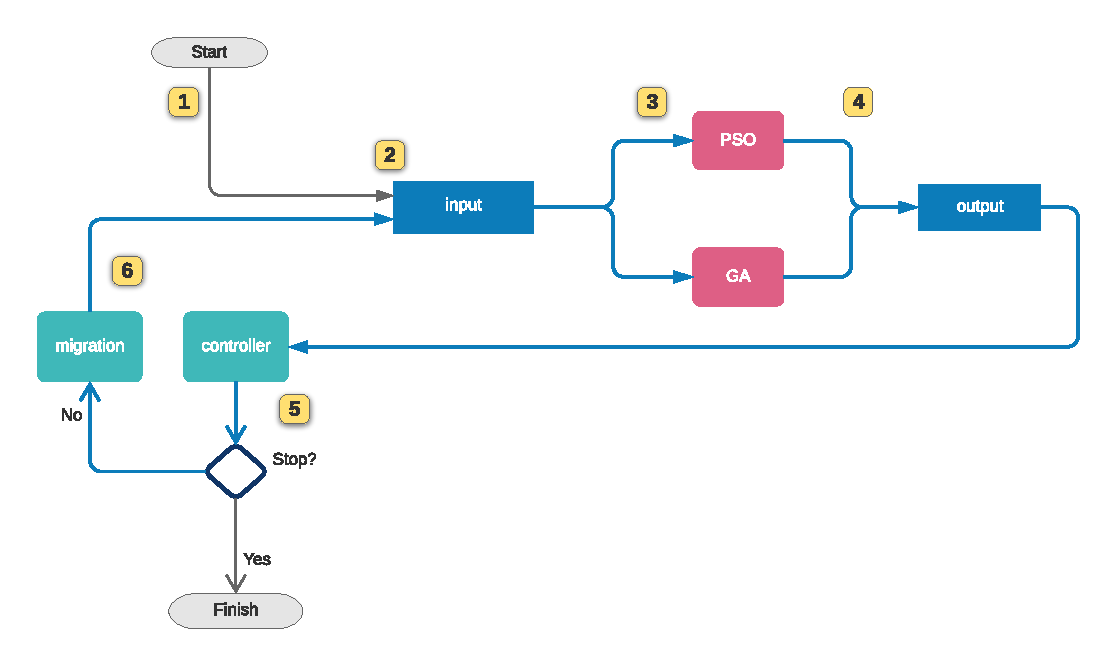
\includegraphics[width=5in]{kafkeo}
\caption{A sample black and white graphic
that needs to span two columns of text.}
\label{fig:kafkeo}
\end{figure*}

\section{Proposed Method}
\label{method}

\subsection{Architecture}
\label{arch}

In this section, present our proposed model for the execution of
multi-population based asynchronous algorithms. As we mention before, when
designing efficient multi-population algorithms, we need to consider additional
issues \cite{Ma2019}, including the number and size of populations, how they
interact between them, and the search strategy and parametrization of
populations. We have considered these requirements and propose a cloud-native
multi-population solution. In this model, populations are the primary data
structure, and we can consider them as messages in a continuous stream flowing
from one algorithm to the other. To achieve this ``continuous stream,''
everything must happen asynchronously without components needing to wait for
others. We implement this streaming functionality by using a message queue
system. Figure \ref{fig:kafkeo} shows the general architecture. We can explain
the model by using an analogy of producers and consumers of messages. There are
two queues, one labeled \texttt{input}, and the other one \texttt{output}. In a
queue, {\em push} operations are represented by solid arrows connecting to the
left side and pull or pop operations as solid arrows leaving from the right
side. The \texttt{controller} process, is responsible for the migration of
individuals from one population to the other, and keeping track of the
iterations of the algorithm. There is at least one \texttt{stateless Function}
worker process responsible for running the isolated algorithms. The two
processes \texttt{PSO} and \texttt{GA}, are shown.

We can follow the path of messages as follows:

\begin{enumerate}

\item In this step, the specified number of populations are created according
to the configuration. Populations at this moment are just static data messages,
including each individual inside. Each population includes a metadata section
where its algorithm and execution parameters are specified. For instance, for a
GA, the mutation rate, type of crossover operator, and other values are
indicated.

\item The setup process pushes each population to the \texttt{input}
queue so that they can be consumed by stateless functions responsible for the
execution of the search.


\item One or more \texttt{stateless functions} are constantly pulling
population messages from the \texttt{input} queue. These functions have the
task of executing the optimization algorithm. They take the current state of
the population and start to run the specified algorithm for a certain number of
iterations.

\item Once they finish the execution, the resulting populations are pushed to
the \texttt{output} queue. Once finished, it pulls another population from the
queue.

\item The \texttt{controller} pulls populations from the \texttt{Output} queue,
inspects the metadata describing the current state of the populations, and if
the algorithm has found an optimal solution or the maximum number of iteration
has been reached it stops the execution.

\item Otherwise, it passes the stream of messages to a migration function,
where populations are mixed. Migration generates new populations, and they are
again pushed to the \texttt{input} queue to continue in a loop. The
\texttt{controller} is also responsible for logging the metadata.

\end{enumerate}

This reactive architecture has the following advantages:
\begin{itemize}

\item It decouples the population and the population-based algorithm. In this
design, we can have one or many processing nodes, each running a different
search strategy.

\item Also, the reactive controller gives designers more control over the
multi-population algorithm. In this process, designers can dynamically change
the number of populations, population parameters, and migration details
on-the-fly.

\item Another advantage is that algorithm designers have many options for
implementing this simple architecture. The same basic components can be
implemented as a single multi-threaded program, or as a highly scalable
serverless cloud application.
\end{itemize}

\subsection{Stateless functions} 
\label{functions} 

This message queue pattern is an essential component of a highly scalable
reactive architecture; one of the reasons for this scalability is the use of
stateless functions that have no secondary effects, or the need to read data
from an external entity. Stateless functions do not need to read, keep, or
modify data outside of the method. If we implement population-based
optimizarion algorithms using stateless functions, then to the system, there is
no difference between having one or many copies of the same function pulling
work from the queue all at the same time, because there are no unwanted side
effects, including problems of resource locking resulting from this
concurrency.

\subsection{Migration}
\label{migration}
%% TO DO:
%% Explain migration

The   \texttt{buffer\_with\_count(3)} operator, waits until it receives 
three valid messages to emit a single message that contains a list with
the previous three. The \texttt{population\_mixer}  method requires that list to mix them. 
In our previous work, we needed a local buffer for storing a certain 
number of populations to mix them with others. This design has the advantage
of not needing extra memory, and it integrates better with the reactive paradigm.
A possible disadvantage can be that it only mixes contiguous populations,
but this can be mitigated with a larger buffer.

The \texttt{population\_mixer} receives a list of three populations,
let us say [A, B, C], and calls the migration method shown in
Algorithm \ref{alg:migration}  for [A, B], [B, C] and [A, C]. 
The migration algorithm sorts both populations and generates
a new population containing the best half from each.
Finally, the method pushes the new populations to the 
\texttt{messages Observable}. From there, a
\texttt{publish(population)} observer is responsible for pushing
the newly generated populations back to the \texttt{Input} message queue.

\begin{algorithm}
    \caption{Migration}
    \label{alg:migration}
    \begin{algorithmic}[1]
        \Procedure{cxBestFromEach}{$pop_1,pop_2$}
            \State $pop_1.sort()$
            \State $pop_2.sort()$
            \State $size\gets min(len(pop_1), len(pop_2))$
            \State $cxpoint\gets (size-1)/2$
            \State $pop_1[cxpoint:]\gets pop_2[:cxpoint+2]$
            \State \textbf{return} $pop_1$
        \EndProcedure 
    \end{algorithmic}
\end{algorithm}



\section{Setup}
\label{setup}

In this section, we verify if having a multi-population algorithm, with
heterogeneous populations and the support for mixing search strategies,
increases the performance of the search by needing fewer function evaluations
than a homogeneous setting.

For the experiment, we used five benchmark separable functions ($f_1 to f_5 $)
from the Continuous Noiseless BBOB testbed, which is part of the Comparing
Continuous Optimizers (COCO) framework \cite{hansen2016coco}. The functions are
real-parameter, single-objective benchmark functions. We tested with fifteen
instances of each function, each having a different optimal value. The standard
benchmark of the testbed uses these 15 instances over 2, 3, 5, 10, 20, and 40
dimensions. With the maximum number of function evaluations (\#FEs) increasing
with the dimension (D), using the expression $10^5 \cdot D$ (i.e. for $D = 2$,
\#FEs is $200,000$).

The COCO framework offers several tools to compare the performance of
algorithms, generating data sets, tables, and reports for an experiment, we
compared using the average required time (aRT). There is a
repository\footnote{\url{https://coco.gforge.inria.fr/doku.php?id=algorithms-bbob}}
of more than 200 results for the noiseless BBOB testbed, collected from BBOB
workshops and special sessions between the years 2009 and 2019. To test the
heterogeneous multi-population capabilities, we compare the aRT between a
homogeneous and an ensemble of multi-populations, using Genetic Algorithms
(GAs) and Particle Swarm Optimization (PSO). We used the DEAP framework for the
GA stateless function \cite{fortin2012deap} and the EvoloPy library
\cite{faris2016evolopy} for the PSO algorithm function. We show the parameters
for each algorithm, in Tables \ref{tab:GAparams} and Table \ref{tab:PSOparams}
for the GA and PSO, respectively. We obtained these parameters by following a
method we used in a previous work \cite{garcia2017benchmarking}. First, we
tested the parameters for the Rastrigin separable function with five
dimensions. After about fifteen experiments, the most challenging targets were
achieved for this particular function. We tested again with functions one to
three, and after obtaining favorable results, we set the PSO and GA algorithm
parameters. We set the mutation and crossover probabilities of the GA randomly
to have heterogeneous populations; the table shows the range of these
parameters. We did not change these settings during the experiments, and we
only provided the population size and number of generations as parameters.

\section{Results}
\label{results}

\begin{table}
    \small
    \caption{ DEAP GA EvoWorker Parameters }
    \label{tab:GAparams} 
    \centering
    \small
    \begin{tabular}{|l|c|}
      \hline
      Selection & Tournament size=12                            \\ \hline
      Mutation & Gaussian $\mu=0.0$, $\sigma=0.5$, indbp=0.05   \\ \hline
      Mutation Probability & [0.1,0.3]                          \\ \hline
      Crossover & Two Point                                     \\ \hline
      Crossover Probability  & [0.2,0.6]                          \\ \hline
    \end{tabular}
  \end{table}
  
  \begin{table}
    \small
    \caption{ EvoloPy PSO Parameters }
    \label{tab:PSOparams} 
    \centering
    \small
    \begin{tabular}{|l|c|}
      \hline
      $V_{max}$ & 6 \\ \hline
      $W_{max}$ & $0.9$ \\ \hline
      $W_{min}$ & $0.2$ \\ \hline
      $C_1$ & 2 \\ \hline
      $C_2$ & 2 \\ \hline
    \end{tabular}
  \end{table}


  \begin{table}
    \small
    \caption{Parameters used in the experiments with ten populations
    }
    \label{tab:params:10}
    \vspace{0.25cm}
    \centering
    \small
    \begin{tabular}{|l|c|c|c|c|c|c|}
      \hline
      Dimension        & 2  & 3  & 5  & 10 & 20  & 40  \\ \hline
      Generations      & 40 & 25 & 28 & 50 & 66  & 80  \\ \hline
      Population Size  & 50 & 60 & 60 & 70 & 100 & 125 \\ \hline
      Populations      & 10 & 10 & 10 & 10 & 10  & 10  \\ \hline
      Iterations       & 10 & 20 & 30 & 30 & 30  & 40  \\ \hline  
    \end{tabular}
\end{table}


% \subsection{Experiment}
% \label{sec:exp_results}
% Having a multi-population based algorithm can decrease the execution time
% because of the parallel execution of the evolution. But, having heterogeneous 
% populations might enhance evolutionary search and needless
% evaluations than homogeneous systems; heterogeneous settings, if
% done right, increases the diversity of the whole population
% \cite{araujo2008multikulti}.

% But this is a rule of thumb, and it will depend on the degree of heterogeneity,
% as well as on the algorithm itself. Some level of heterogeneity can be
% implemented by just changing the configuration parameters of each population,
% but in this case, we are interested in a heterogeneous search strategy. 
% Therefore, in this experiment we compare a multi-population with only GA and PSO populations,
% versus an ensemble of GA and PSO algorithms. We tested on the first five functions of the
% BBOB testbed. We used ten populations and eight workers for the experiment and the
% same parameters as before.  


\begin{figure*}[h!tb]
    \begin{tabular}
        {c@{\hspace*{-0.00001\textwidth}}
         c@{\hspace*{-0.00001\textwidth}}
         c@{\hspace*{-0.00001\textwidth}}
        }
    GA  &  PSO & GA \& PSO\\   
    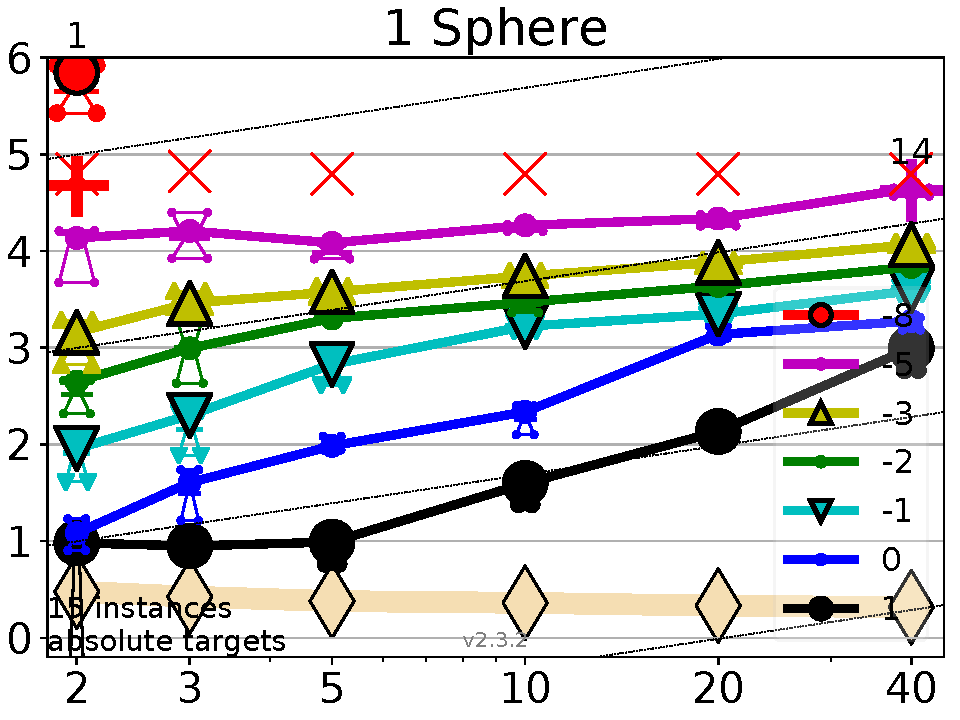
\includegraphics[width=0.28\textwidth]{GAOnly_f001}&
    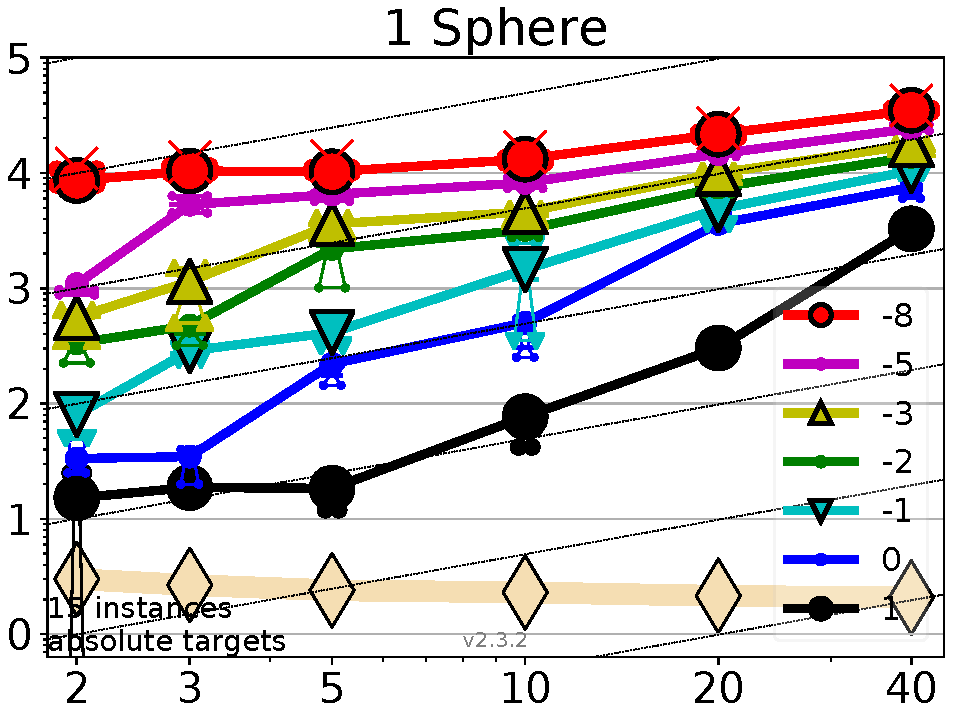
\includegraphics[width=0.28\textwidth]{PSOOnly_f001}&
    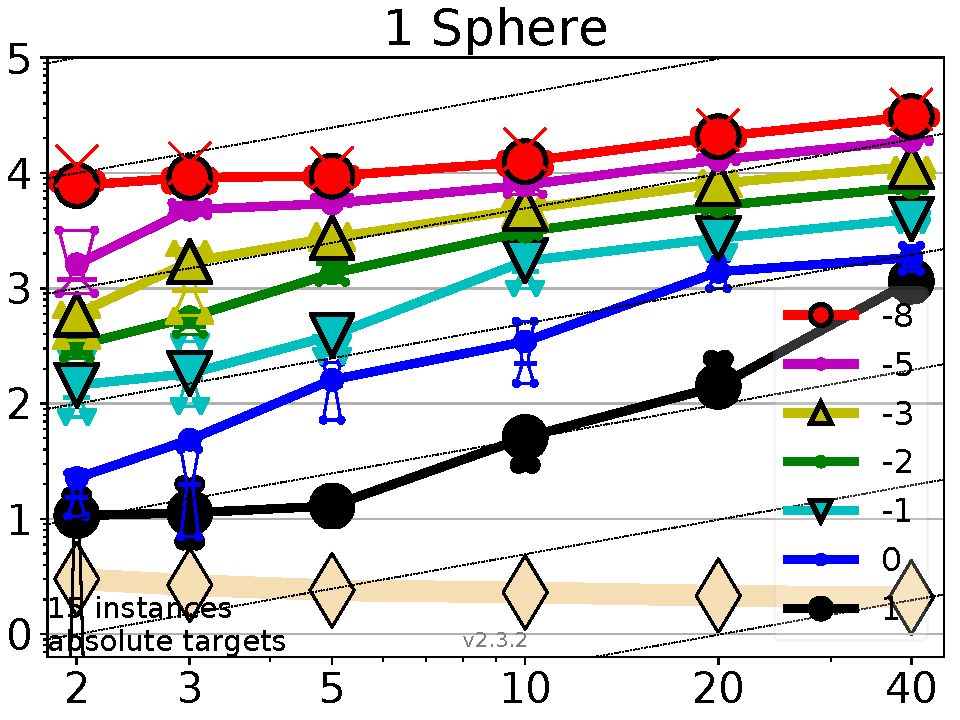
\includegraphics[width=0.28\textwidth]{GAPSO_f001}\\

    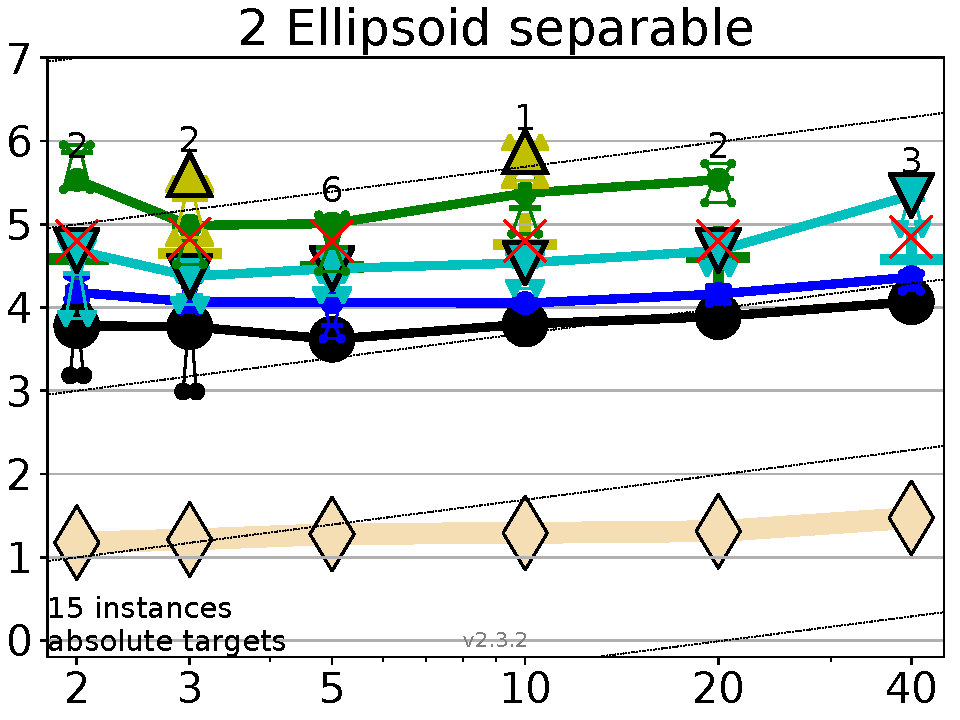
\includegraphics[width=0.28\textwidth]{GAOnly_f002}&
    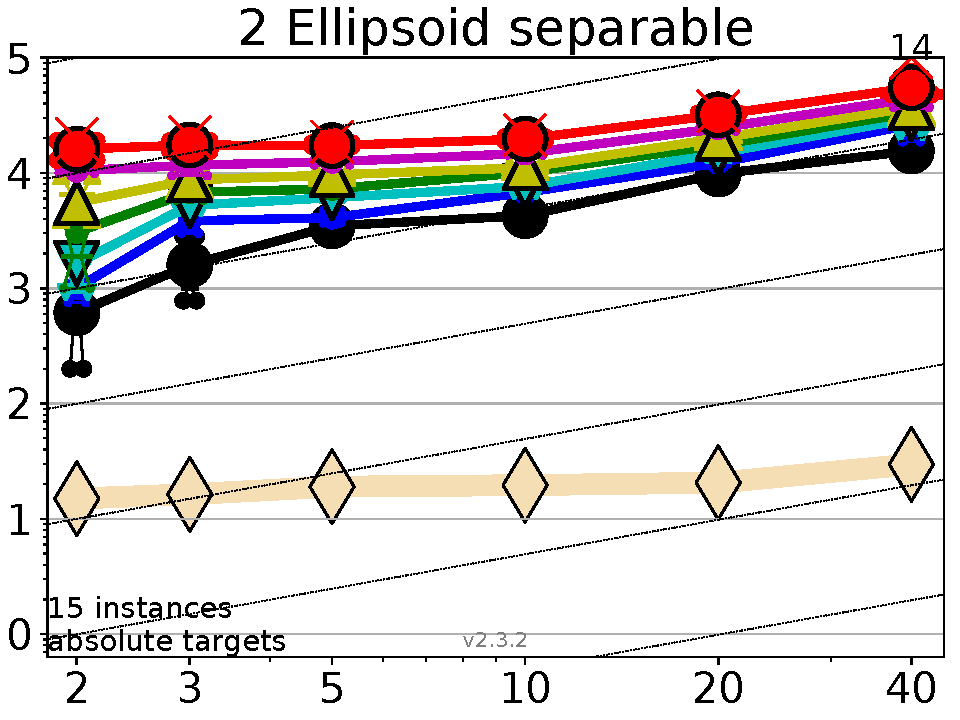
\includegraphics[width=0.28\textwidth]{PSOOnly_f002}&
    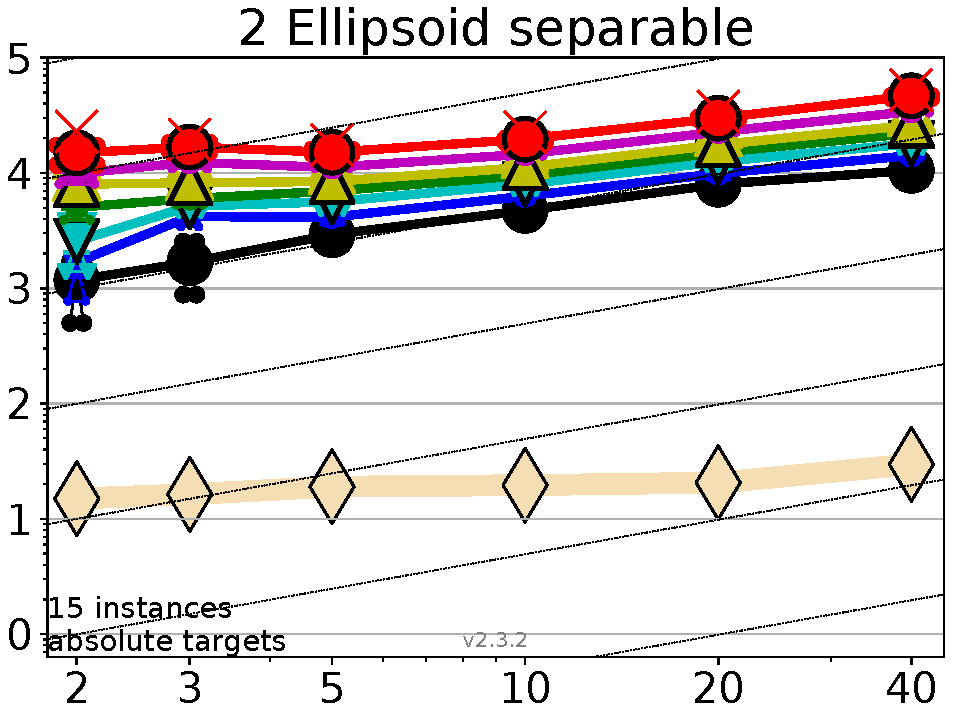
\includegraphics[width=0.28\textwidth]{GAPSO_f002}\\

    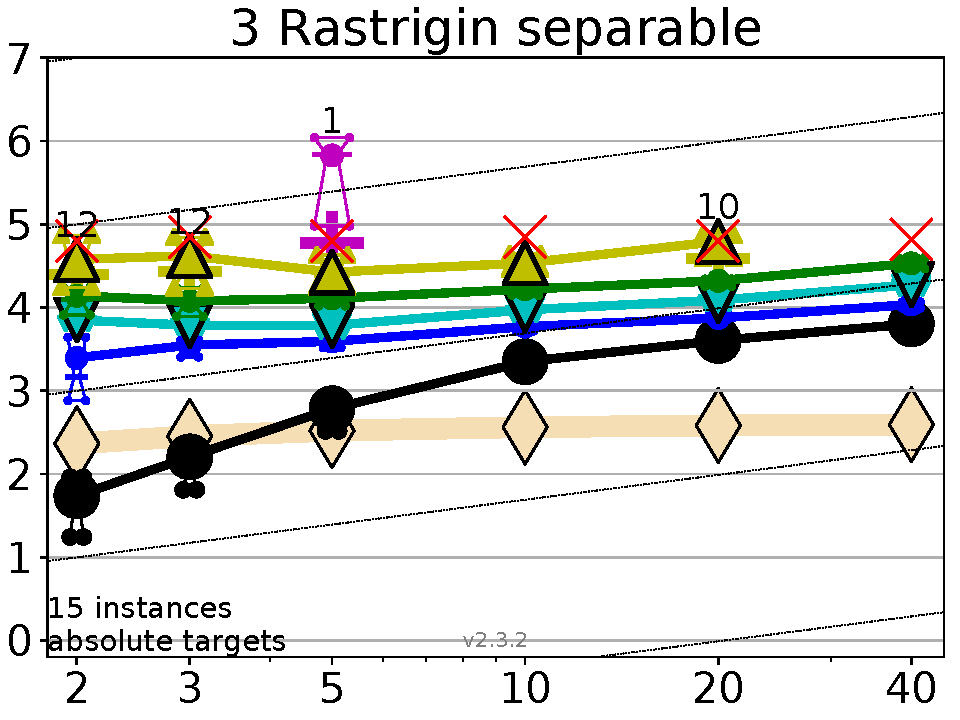
\includegraphics[width=0.28\textwidth]{GAOnly_f003}&
    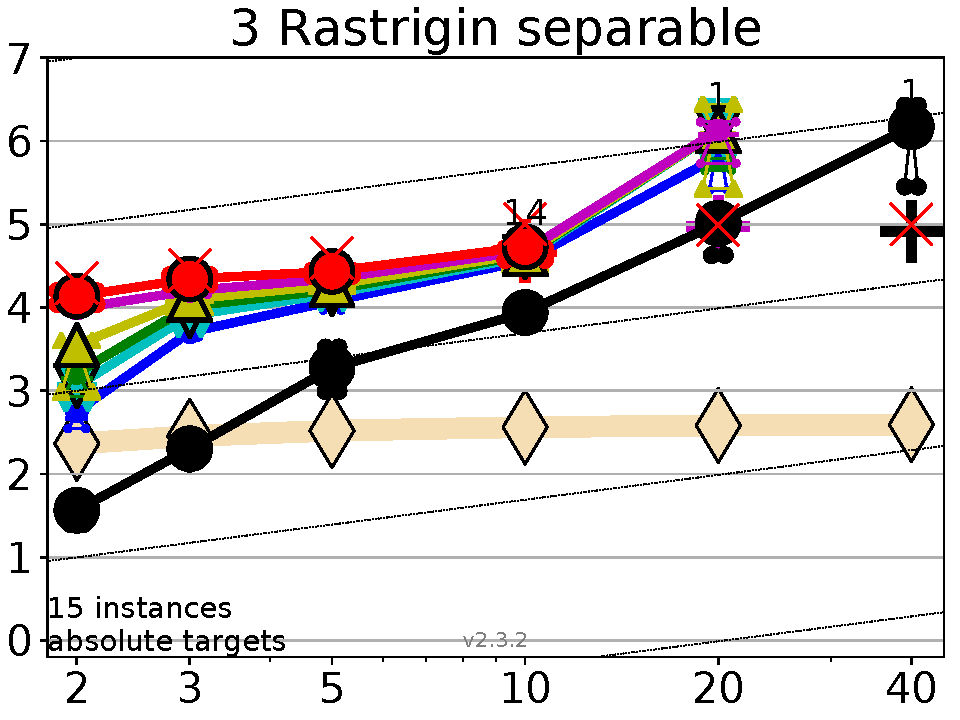
\includegraphics[width=0.28\textwidth]{PSOOnly_f003}&
    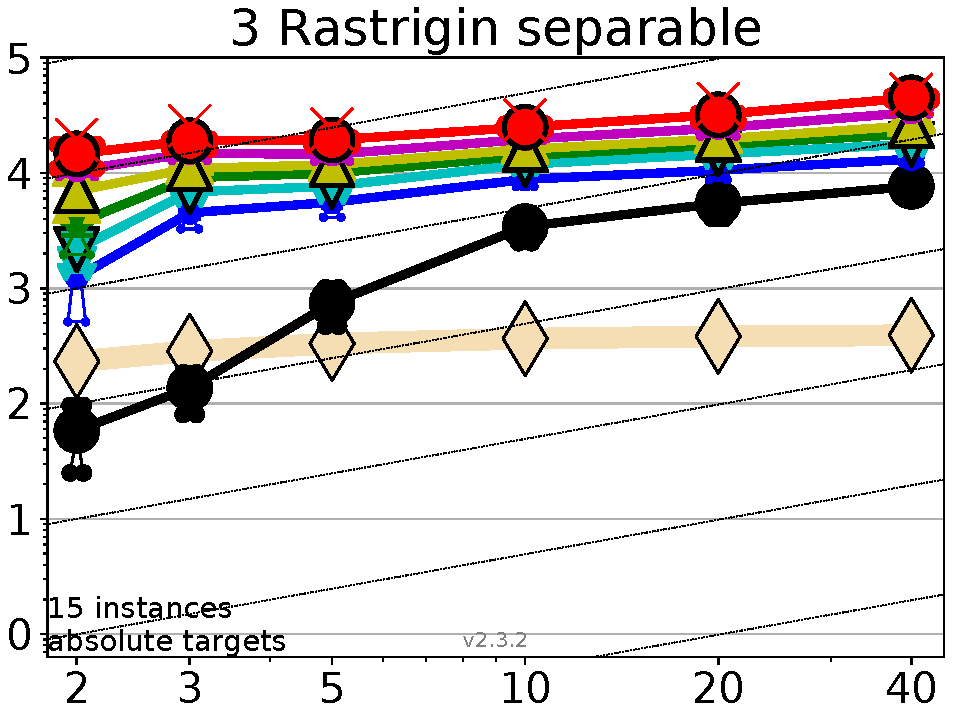
\includegraphics[width=0.28\textwidth]{GAPSO_f003}\\

    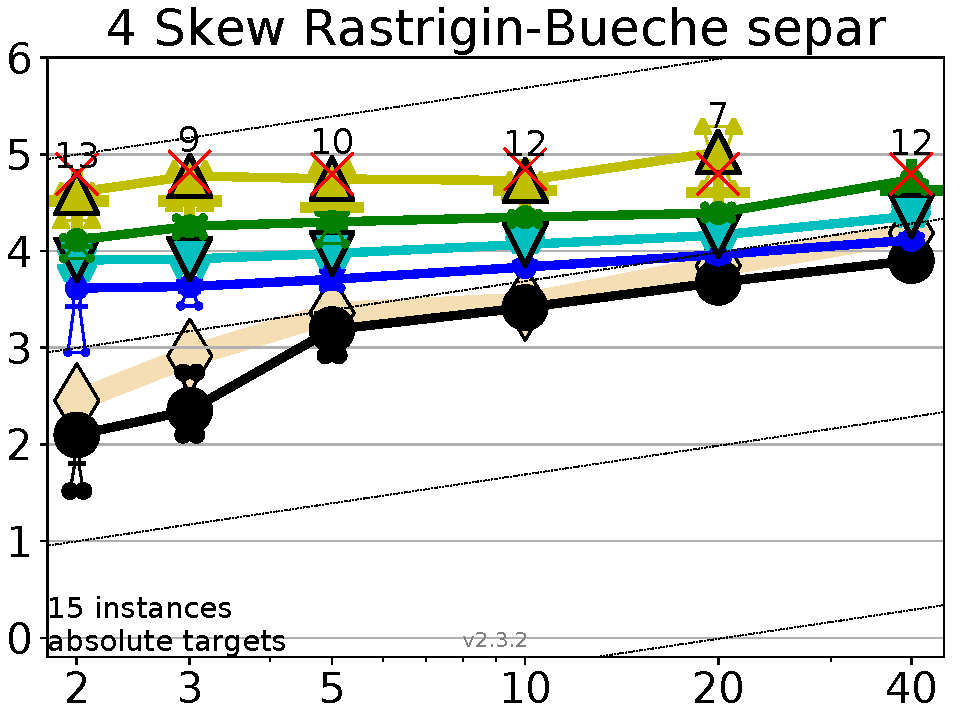
\includegraphics[width=0.28\textwidth]{GAOnly_f004}&
    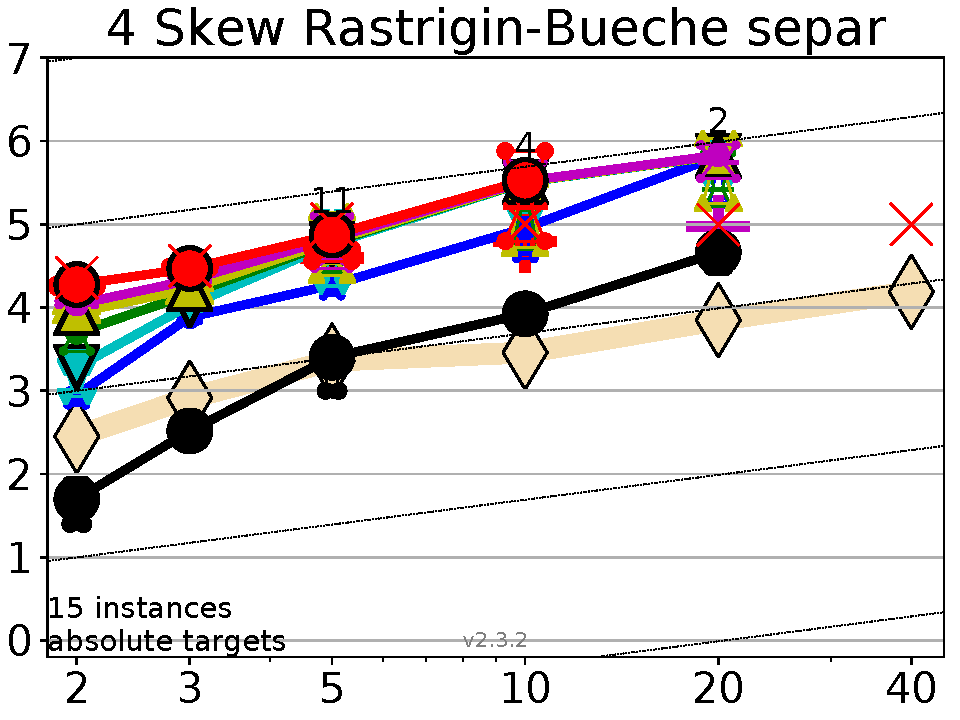
\includegraphics[width=0.28\textwidth]{PSOOnly_f004}&
    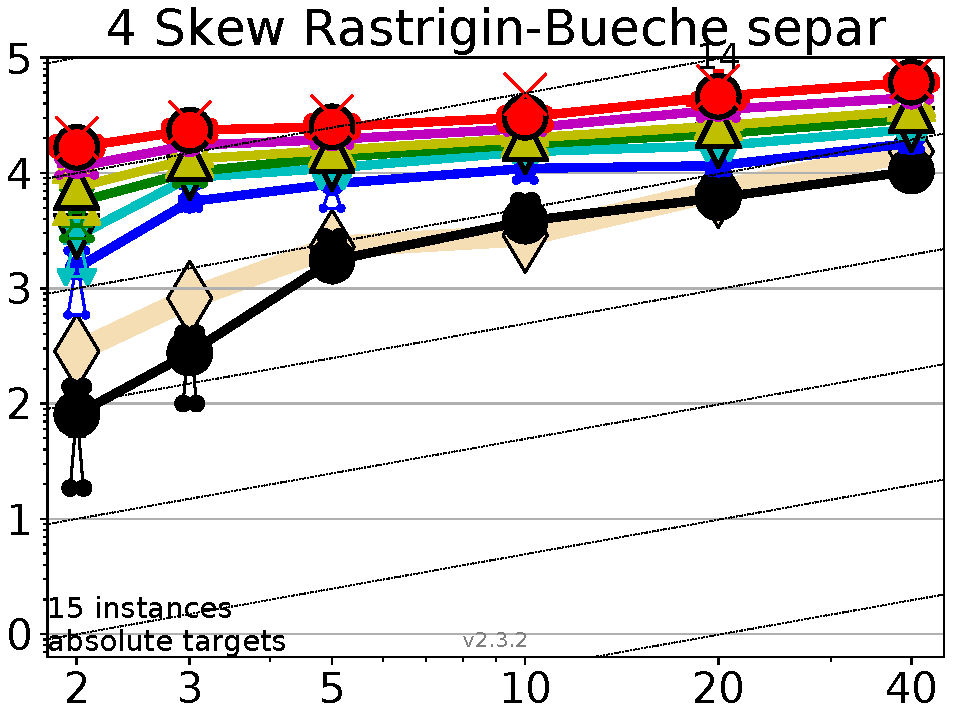
\includegraphics[width=0.28\textwidth]{GAPSO_f004}\\

    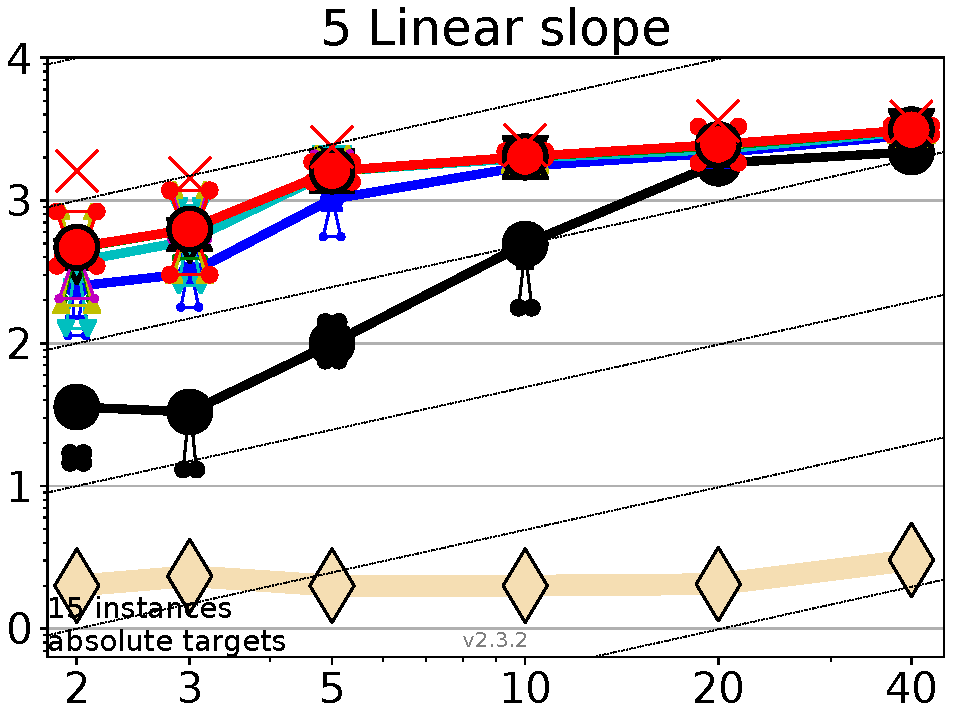
\includegraphics[width=0.28\textwidth]{GAOnly_f005}&
    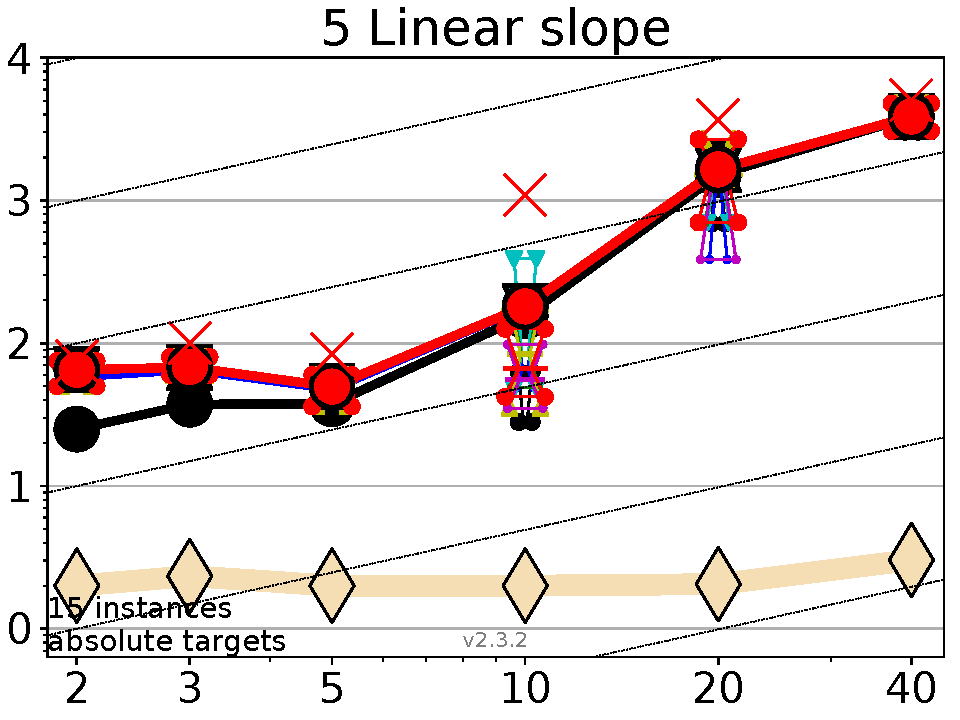
\includegraphics[width=0.28\textwidth]{PSOOnly_f005}&
    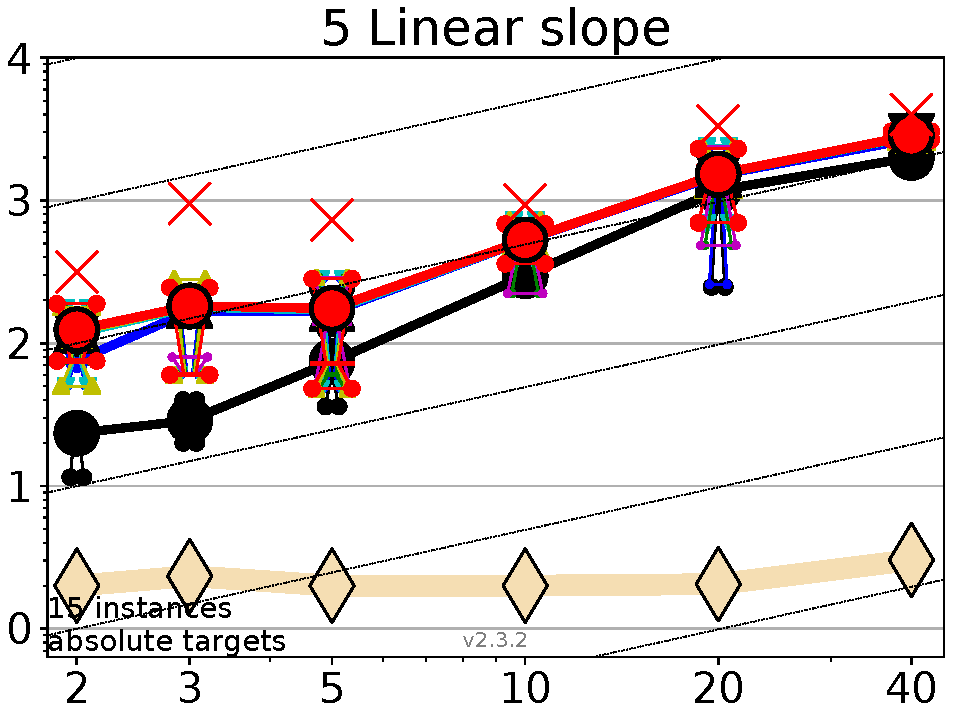
\includegraphics[width=0.28\textwidth]{GAPSO_f005}\\
    \end{tabular}
    \vspace{-3ex}
     \caption{
 Scaling of runtime with dimension to reach certain target values $\Delta f$. Lines:
 average runtime (aRT); Cross ($+$): median runtime of successful runs to reach
 the most difficult target that was reached at least once (but not always);
 Cross (\textcolor{red}{$\times$}): maximum number of f-evaluations in any trial. Notched boxes:
 interquartile range with median of simulated runs; All values are divided by
 dimension and plotted as $log_{10}$ values versus dimension. 
 %Shown is the aRT for
 %fixed values of $\Delta f = 10k$ with $k$ given in the legend. 
 Numbers above aRT-symbols
 (if appearing) indicate the number of trials reaching the respective target.
 %The light thick line with diamonds indicates the best algorithm from BBOB 2009
 %for the most difficult target. Horizontal lines mean linear scaling, slanted
 %grid lines depict quadratic scaling.
 }
\end{figure*}


    \begin{figure}[h!tb]
        \begin{tabular}
            {c@{\hspace*{-0.00001\textwidth}}
            % c@{\hspace*{-0.00001\textwidth}}
            }
           
        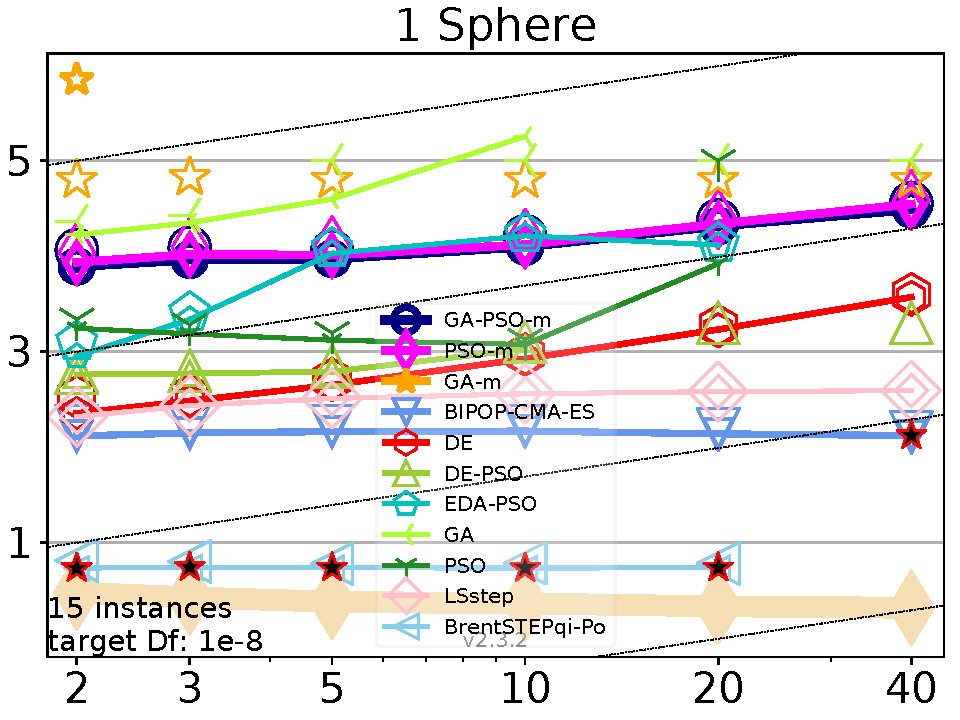
\includegraphics[width=0.28\textwidth]{ppfigs_f001}\\
        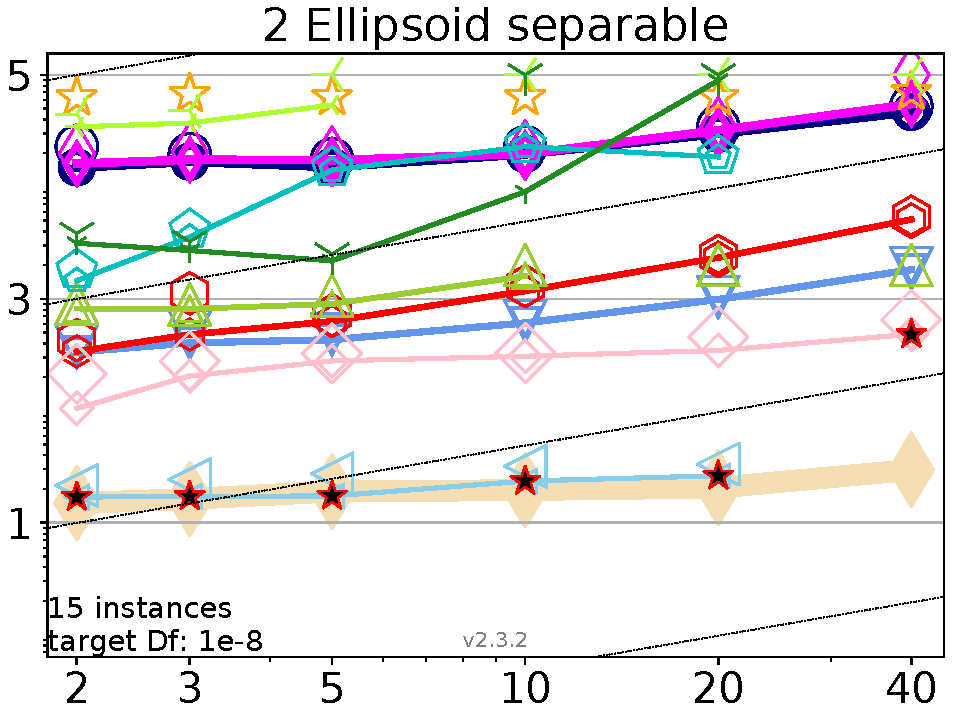
\includegraphics[width=0.28\textwidth]{ppfigs_f002}\\

        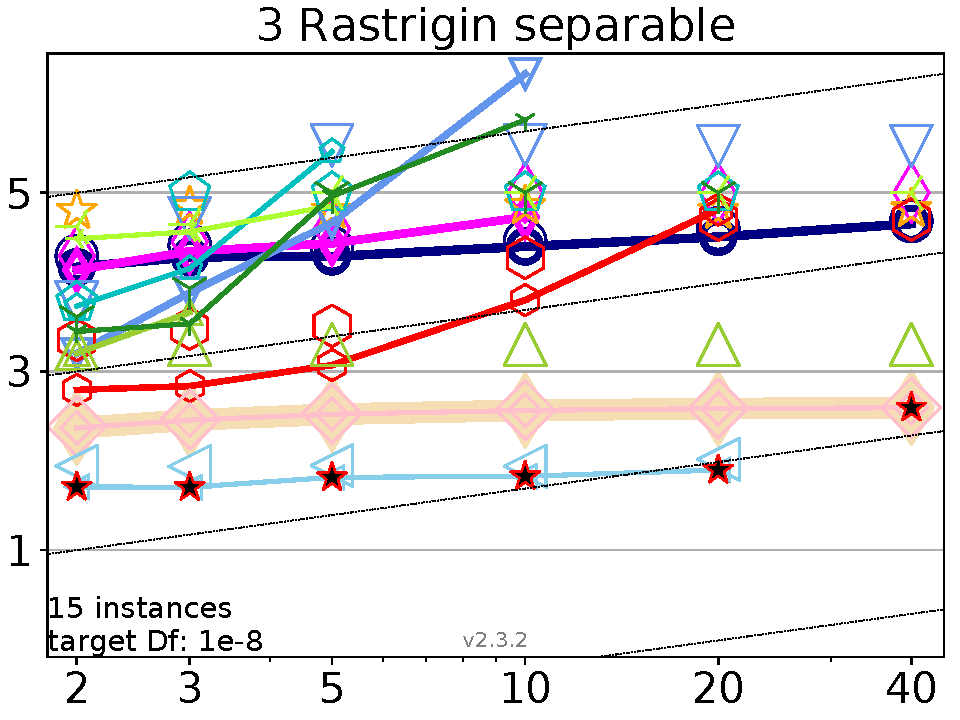
\includegraphics[width=0.28\textwidth]{ppfigs_f003}\\
        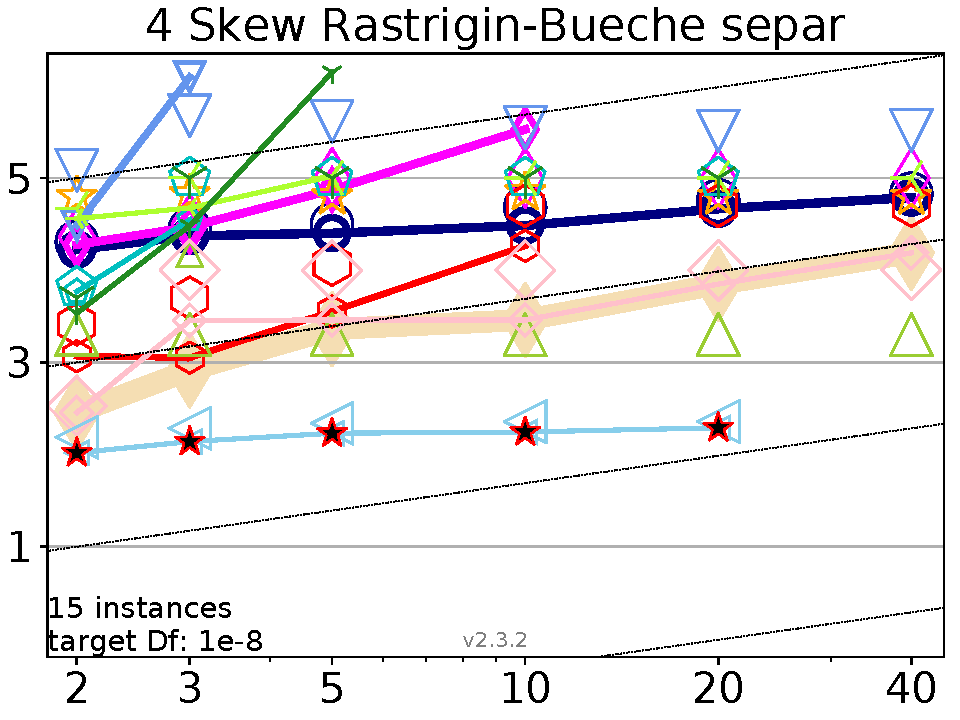
\includegraphics[width=0.28\textwidth]{ppfigs_f004}\\
        
        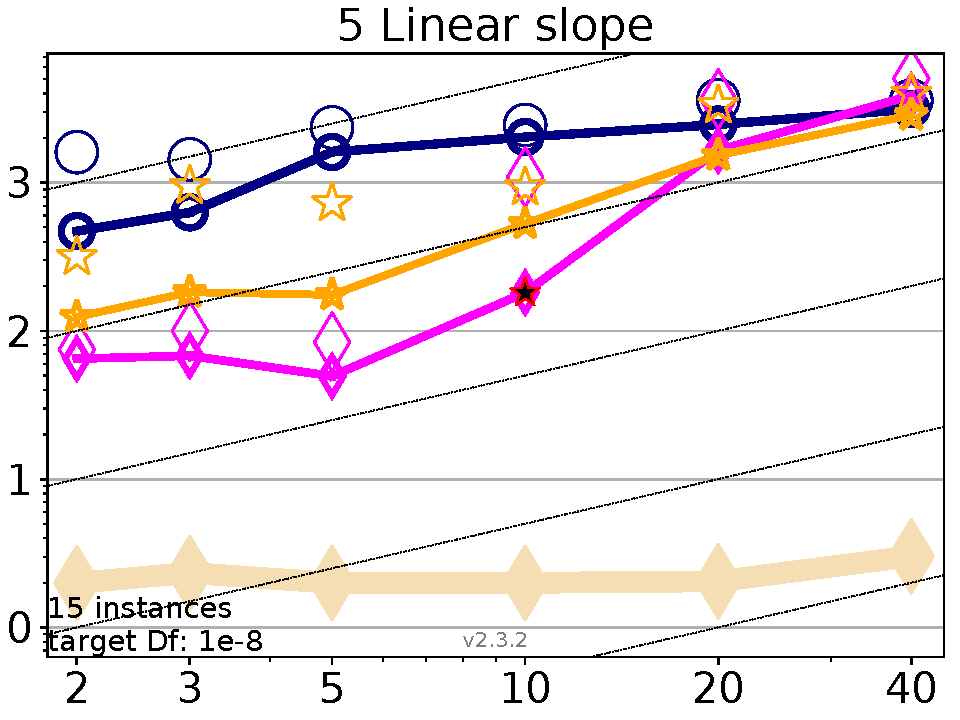
\includegraphics[width=0.28\textwidth]{ppfigs_f005}\\
        \end{tabular}
        \vspace{-3ex}
         \caption{Average running time (in \#FEs as $log_{10}$ value),
          divided by dimension for target function value $10^{-8}$ vs dimension. 
          Algorithms legends are given in $f_1$. Light symbols give the maximum number of 
          function evaluations from the longest trial divided by dimension. 
          Black stars indicate a statistically better result compared to 
          all other algorithms ($p < 0.01$) and Bonferroni 
          correction number of dimensions (six).}
    \end{figure}  

\section{Conclusions}
\label{conclusions}

\begin{acks}

  The authors would also like to thank the anonymous referees for
  their valuable comments and helpful suggestions. The work is
  supported by the 
\end{acks}


\bibliographystyle{ACM-Reference-Format}
\bibliography{multipopulation,hybrid} 

\end{document}
